\subsection{版本与扩展验证}
CPU主实验保留0.1.0源代码和原协议；0.1.1增加约束输出检查、末窗口有效步掩码、错误及失败记录，并修复R单元素数组。变换检查和掩码可能影响计时，不能用旧性能代表新版。审查后对8目标、5工作流各取原较短预算的第一个重复，旧/新源码分别执行；MH复用保存的实际随机数组，NUTS复用锁定随机流。40组均返回有效输出，最大路径差为$1.99\times10^{-13}$，接受事件零失配。这是有限数值对照，不是性能等价或边界正确性证明。

新增Poisson回归示例无需改动内核，公开模型对象分别实现JAX密度与独立NumPy密度/解析梯度，先验证坐标和导数，再比较固定输入的四种MH工作流。密度与梯度最大差约$2.84\times10^{-14}$；MALA和RWM配对最大路径差分别为$7.90\times10^{-11}$和$3.61\times10^{-16}$，接受事件无失配。示例旨在说明扩展和核验，不作为新性能或后验收敛证据。

\subsection{同数据集的解析SBC对照}
本节为审查后伴随分析，未追溯为原协议预声明检验。64组真参数和数据已保存，后验为$N(\sum_j y_j/9,1/9)$，故直接计算解析90\%区间，无需新增拟合。解析区间覆盖54/64，点估计0.84375，95\%二项区间为[0.731,0.922]。五种工作流共享同64组数据，同核顺序/并行还共享轨迹，因此不能当作五次独立校准证据。

\begin{table}[htbp]\centering\small\setlength{\tabcolsep}{4pt}
\begin{tabular}{lrrrrrr}\toprule
工作流 & 覆盖数 & 分歧数 & 下端点RMSE & 上端点RMSE & 均值RMSE & 标准差RMSE\\\midrule

顺序MALA & 54 & 4 & 0.0179 & 0.0195 & 0.0105 & 0.0063\\

quasi-DEER & 54 & 4 & 0.0179 & 0.0195 & 0.0105 & 0.0063\\

顺序RWM & 53 & 3 & 0.0318 & 0.0267 & 0.0147 & 0.0107\\

Picard & 53 & 3 & 0.0318 & 0.0267 & 0.0147 & 0.0107\\

NUTS & 53 & 3 & 0.0222 & 0.0190 & 0.0115 & 0.0078\\

\bottomrule\end{tabular}
\caption{同64数据集的配对解析对照。RMSE按数据集计算；分歧指解析与MCMC区间对同一真参数的覆盖判断不同，不能只据总体覆盖率相等判定区间相等。}
\end{table}
MALA的分歧数据集编号为23、32、36、56，RWM为26、32、56，NUTS为11、26、36（从0编号）。例如MALA有2例解析覆盖而MCMC未覆盖、另2例相反，抵消后总覆盖数相同。该批解析覆盖本身偏低，与有限生成样本波动的解释相容；端点及后验矩误差仍显示有限链估计差异，不能据此证明无额外采样偏差。

\subsection{现代诊断与有限预算误差的对应}
从全部1920项保存样本及8次参考拟合提取每个参数和预声明函数，以posterior 1.7.0计算秩正态化/折叠split-$\hat R$、bulk ESS与tail ESS\cite{posterior}。每个拟合分别计算，结果不替换原经典函数诊断；常量链等不可判定值保留为空。表中汇总NUTS，全80组的逐拟合、逐变量诊断随复现材料交付。

\begin{table}[htbp]\centering\scriptsize
\begin{tabular}{lrrrrrrl}\toprule
目标/$N$ & 发散\% & 上限\% & 最大$\hat R$ & 最小bulk ESS & 最小tail ESS & 函数误差 & 判据\\\midrule

A1/256 & 0.00 & 0.00 & 1.018 & 496.4 & 469.7 & 0.00243 & 低于阈值\\

A1/2048 & 0.00 & 0.00 & 1.002 & 5576.0 & 5186.4 & 0.000665 & 低于阈值\\

G1/256 & 0.00 & 0.00 & 1.018 & 1198.4 & 461.8 & 0.00271 & 低于阈值\\

G1/2048 & 0.00 & 0.00 & 1.003 & 11148.1 & 5316.6 & 0.000531 & 低于阈值\\

G2/256 & 0.00 & 0.00 & 1.015 & 636.5 & 448.0 & 0.00383 & 低于阈值\\

G2/2048 & 0.00 & 0.00 & 1.002 & 5848.5 & 5429.4 & 0.000322 & 低于阈值\\

H1/256 & 0.71 & 2.67 & 1.745 & 6.3 & 8.0 & 0.154 & 高于阈值\\

H1/2048 & 1.11 & 3.16 & 1.273 & 11.4 & 5.4 & 0.112 & 高于阈值\\

H2/256 & 0.00 & 0.00 & 1.018 & 815.5 & 545.5 & 0.000595 & 低于阈值\\

H2/2048 & 0.00 & 0.00 & 1.002 & 7125.8 & 5438.9 & 6.11e-05 & 低于阈值\\

L1/256 & 0.00 & 0.00 & 1.017 & 358.2 & 393.2 & 0.000154 & 低于阈值\\

L1/2048 & 0.00 & 0.00 & 1.003 & 3459.7 & 4381.6 & 1.46e-05 & 低于阈值\\

L2/256 & 0.00 & 0.00 & 1.019 & 507.4 & 532.0 & 3.52e-06 & 不可判定\\

L2/2048 & 0.00 & 0.00 & 1.002 & 4243.8 & 5109.4 & 2.28e-07 & 不可判定\\

M1/256 & 0.00 & 0.00 & 1.738 & 6.2 & 30.6 & 0.301 & 高于阈值\\

M1/2048 & 0.00 & 0.00 & 1.734 & 6.1 & 26.8 & 0.296 & 高于阈值\\

\bottomrule\end{tabular}
\caption{NUTS按模型和保留预算分组的伴随诊断。发散和上限命中以24次拟合、各4链的全部保留转移为分母；$\hat R$为参数与拟合中的最大值，ESS为最小值。函数误差为原预声明最大平方误差/参考平方差，判据对应原逐点95\%区间与0.01阈值，不由诊断阈值重定义。}
\end{table}
2358次发散与6861次积分上限命中均来自中心化漏斗H1：短/长预算分别为174/2184次发散及657/6204次上限命中。双峰M1无发散，却在两个预算下都有约1.73的最大参数$\hat R$，所选函数误差亦高于阈值。五个目标的长预算函数误差区间低于阈值，与H1/M1的探索问题分别成立；L2参数诊断良好不消除参考符号事件恒零的不确定性。特定函数误差小、无发散和后验全面探索是不同陈述。

\subsection{三种成本口径}
缓存执行衡量已编译内核；正常推断应包含必要建模、编译、预热、转换及诊断；研究审计另加入独立顺序参考和完整数组、校验和归档。历史时钟未单独测量正常输出与所有建模步骤，故只能以$T_{\rm API}-T_{\rm independent}+T_{\rm diagnostic}$给出内存内正常使用的记账估计，不能冒称重新实测的完整正常工作流。该估计不含未分离的建模、R转换和持久化费用。

\begin{table}[htbp]\centering\small\setlength{\tabcolsep}{4pt}
\begin{tabular}{lrrr}\toprule
执行器 & 缓存执行 & 正常内存口径估计 & 研究审计工作流\\\midrule

quasi-DEER & 0.019--0.174 & 0.038--0.175 & 0.072--0.739\\

Picard & 0.050--0.809 & 0.110--0.393 & 0.226--0.814\\

\bottomrule\end{tabular}
\caption{历史主实验中，各模型--预算组的配对速度比中位数范围。三列均为顺序时间/并行时间；中列是不同包含项的记账敏感性分析，不与另外两列混称三种完整实测工作流。}
\end{table}
共享审计成本使速度比向1靠近，可能掩盖加速或减速；当前缓存与去独立核验的估计口径也均未显示组中位加速，因此负结果不能仅归因于审计。新增机制实验另直接计量\texttt{audit=False}的建模、采样与基本均值/方差/链间诊断，并单列普通样本输出耗时；它是最小Python正常工作流，不包含R转换及现代posterior诊断，也不是全新进程冷启动。

\subsection{小型CPU机制实验}
审查后另冻结\texttt{cpu-mechanism-v1}，使用0.1.1，目标G1/G2/L1、链数1/4、窗口16/64、每链256步、两组成对MH执行方式和每格3个新实际随机数组，共72项任务。沿用主协议的指定核参数，冻结随机顺序；没有按速度追加或删除任务。每次至少7次缓存计时重放、总观测窗口至少0.2秒，作为技术重复而非独立统计重复。全部72项完成；分段重放与生产程序首链的接受事件无失配。

生产执行另外记录进程CPU秒/墙钟秒和10毫秒间隔系统利用率。组中位进程占用约为1.00--2.99个CPU核当量，测量包含运行返回和监测开销，不是物理核心绑定，也不能将\texttt{vmap}当作指定核心数的证明。固定前驱状态的微基准比较串行映射与向量化映射在同一批状态、噪声上的吞吐；它没有MCMC的递推依赖，不能将吞吐比直接当作轨迹加速比。

\begin{figure}[htbp]\centering
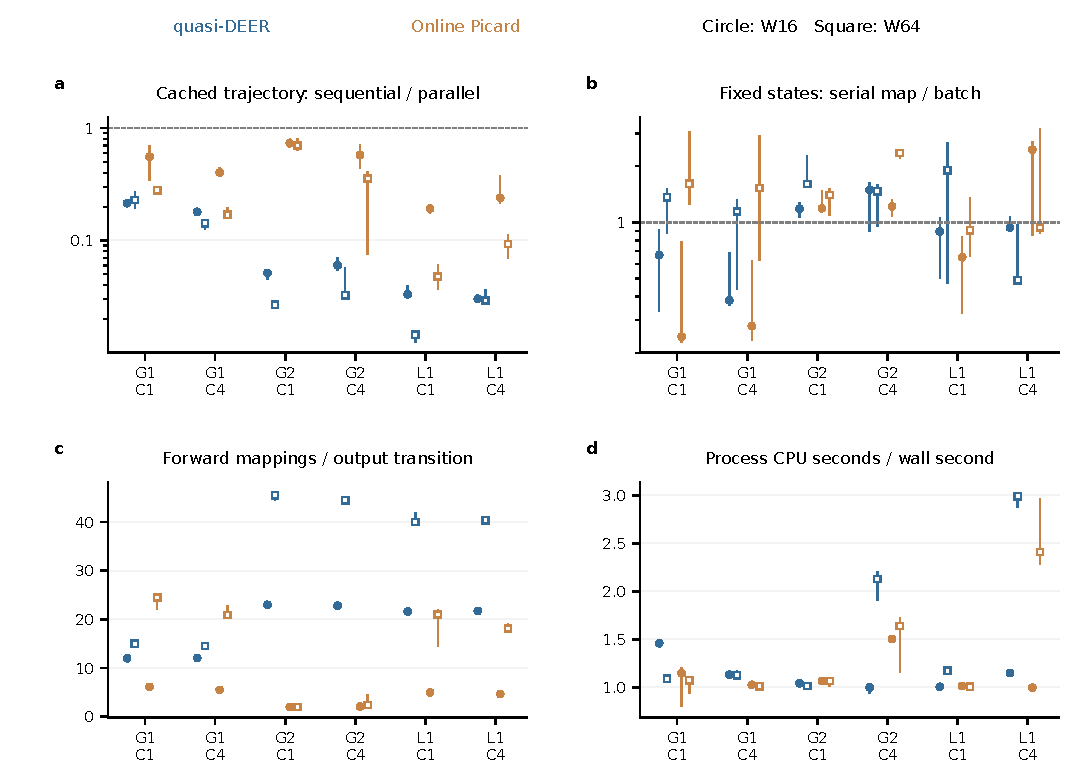
\includegraphics[width=\linewidth]{../../figures/software/cpu-mechanism.pdf}
\caption{新冻结的72项机制任务。每格3个实际随机数组，符号为组中位数，细线为最小至最大值；技术计时重复不扩大样本量。蓝色为quasi-DEER，橙色为Picard；圆点为窗口16，方形为64；横轴C为链数。a：缓存轨迹速度比，1以上才为加速。b：固定状态批量吞吐比，1以上表示批处理有利，但它不是轨迹加速。c：每个输出转移的前向映射求值数，quasi-DEER还另有JVP；拒绝自环计入转移。d：进程CPU秒/墙钟秒，表示观测消费量而非核数配置。}
\end{figure}

quasi-DEER的组中位缓存速度比为0.0145--0.23，固定状态批量吞吐比为0.381--1.91；每转移前向映射数为12--45.5，另有5.5--22.2次JVP。

Picard的组中位缓存速度比为0.0477--0.732，固定状态批量吞吐比为0.244--2.46；每转移前向映射数为2--24.5。

这些量显示局部批量求值收益与完整轨迹重复工作之间的差距，而非证明单一瓶颈。例如G1、四链Picard把窗口从16增至64时，首链每轮确认数的组中位数均约5.57，前向工作却从5.50增至20.88次/转移，缓存速度比由0.402降至0.170。G2、单链quasi-DEER的平均每窗口轮数由11增至22.25，前向工作从23增至45.5次/转移，速度比由0.051降至0.027。窗口扩大会增加可批处理宽度，但确认推进和求解轮数决定有效工作效率；这些例子是冻结小网格中的观察，尚未识别正加速的交叉点。

为审查阶段组成，另将首链实现拆成单独编译的批量求值/JVP、扫描和接受复核，并记录每轮残差或确认前缀。拆分插入同步及Python控制，改变了融合执行。所得控制及未细分部分比例很高，不能据此宣称生产程序主要受Python控制限制；它暴露了分段探针的扰动。全部阶段秒数和原始逐轮记录公开，可用于复查数值过程；对生产程序的精确XLA剖面仍属于局限。三次独立重复及短微基准不足以给出普遍硬件因果结论。

\subsection{可移植复现检查}
另建锁定依赖的Python环境并安装非editable轮子，在迁移目录运行完整测试。首次57项通过、1项因漏带上游比较源文件而失败；补齐许可与该源文件后，仅复查失败项并通过，保留初次失败日志。迁移目录的新目标示例也通过。R包检查日志与显式\texttt{PB\_RUN\_INTEGRATION=1}的3项集成测试日志分别交付，后者实际执行15个断言，不以默认跳过替代通过。

迁移目录从1920项主实验、8次参考拟合和320项SBC原始证据重建主摘要，逐字节一致。三个归档含全部源代码、协议、原始数组和论文输入；新临时目录解压后，校验、分析、1928项现代诊断重算、绘图和编译均通过，诊断值排除耗时后逐项一致。检查仍共享Mac、R库和编译器，不等同外部团队或异构系统复现。

